
% Copyright 2004 by Till Tantau <tantau@users.sourceforge.net>.
%
% In principle, this file can be redistributed and/or modified under
% the terms of the GNU Public License, version 2.
%
% However, this file is supposed to be a template to be modified
% for your own needs. For this reason, if you use this file as a
% template and not specifically distribute it as part of a another
% package/program, I grant the extra permission to freely copy and
% modify this file as you see fit and even to delete this copyright
% notice. 

\documentclass{beamer}

% There are many different themes available for Beamer. A comprehensive
% list with examples is given here:
% http://deic.uab.es/~iblanes/beamer_gallery/index_by_theme.html
% You can uncomment the themes below if you would like to use a different
% one:
%\usetheme{AnnArbor}
%\usetheme{Antibes}
%\usetheme{Bergen}
%\usetheme{Berkeley}
%\usetheme{Berlin}
%\usetheme{Boadilla}
%\usetheme{boxes}
%\usetheme{CambridgeUS}
%\usetheme{Copenhagen}
%\usetheme{Darmstadt}
%\usetheme{default}
%\usetheme{Frankfurt}
%\usetheme{Goettingen}
%\usetheme{Hannover}
%\usetheme{Ilmenau}
%\usetheme{JuanLesPins}
%\usetheme{Luebeck}
\usetheme{Madrid}
%\usetheme{Malmoe}
%\usetheme{Marburg}
%\usetheme{Montpellier}
%\usetheme{PaloAlto}
%\usetheme{Pittsburgh}
%\usetheme{Rochester}
%\usetheme{Singapore}
%\usetheme{Szeged}
%\usetheme{Warsaw}

\title{Image Matching}

% A subtitle is optional and this may be deleted
\subtitle{Session 5}

%\author{F.~Author\inst{1} \and S.~Another\inst{2}}
% - Give the names in the same order as the appear in the paper.
% - Use the \inst{?} command only if the authors have different
%   affiliation.

\institute[Computer Vision Group]
{
  Computer Vision Group\\
  IIT Madras
}
% - Use the \inst command only if there are several affiliations.
% - Keep it simple, no one is interested in your street address.

\date{December 5, 2014}
% - Either use conference name or its abbreviation.
% - Not really informative to the audience, more for people (including
%   yourself) who are reading the slides online

\subject{Theoretical Computer Science}
% This is only inserted into the PDF information catalog. Can be left
% out. 

% If you have a file called "university-logo-filename.xxx", where xxx
% is a graphic format that can be processed by latex or pdflatex,
% resp., then you can add a logo as follows:

% \pgfdeclareimage[height=0.5cm]{university-logo}{university-logo-filename}
% \logo{\pgfuseimage{university-logo}}

% Let's get started
\begin{document}

\begin{frame}
  \titlepage
\end{frame}

\begin{frame}{Outline}
  \tableofcontents
  % You might wish to add the option [pausesections]
\end{frame}

% Section and subsections will appear in the presentation overview
% and table of contents.
\section{Template Matching}

\begin{frame}{Template Matching}
    \centering
        
\includegraphics[width=80mm]{images/p1.png}
\includegraphics[width=10mm]{images/template2.png}

\end{frame}

\begin{frame}{Template Matching}
    \centering
        
\includegraphics[width=80mm]{images/temp_match.png}
\includegraphics[width=10mm]{images/template2.png}

\end{frame}
\begin{frame}{Template Matching}
    \centering
    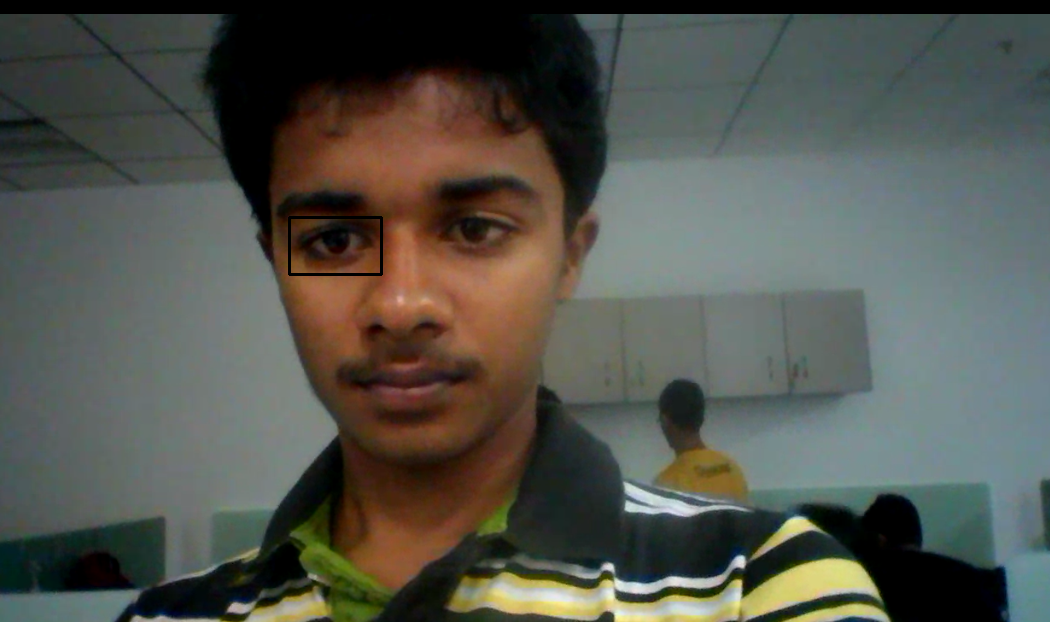
\includegraphics[width=90mm]{images/template_matching.png}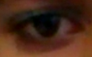
\includegraphics[width=20mm]{images/template1.png}

\end{frame}

\section{Matching using features}
\begin{frame}{Matching using features}
    \centering
        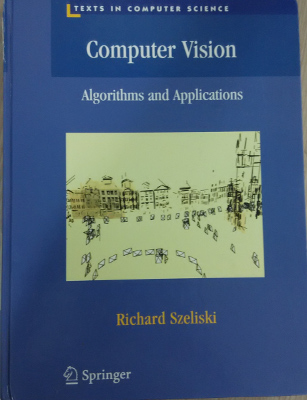
\includegraphics[width=40mm]{images/t2.jpg}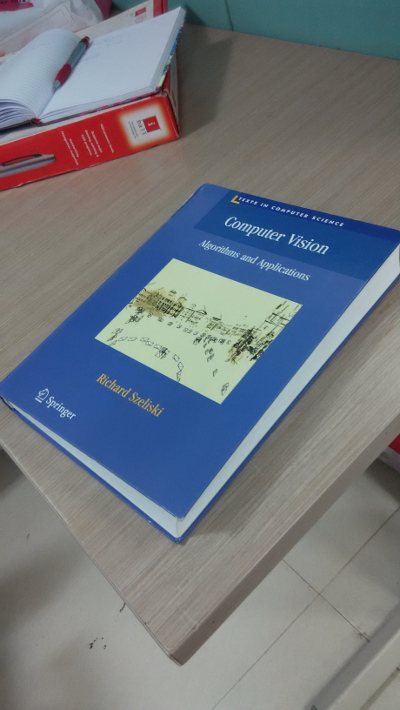
\includegraphics[width=40mm]{images/p2.jpg}

\end{frame}

\begin{frame}{Matching using features}
    \centering
        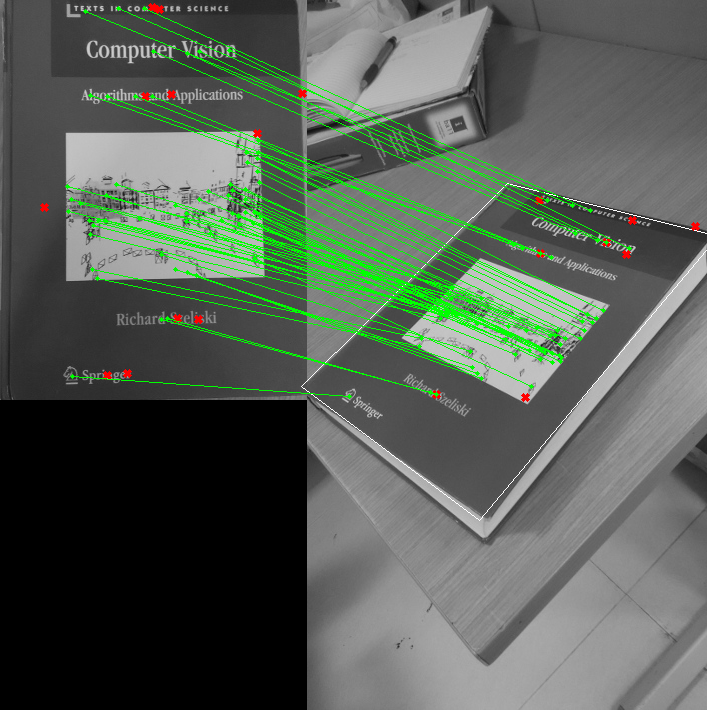
\includegraphics[width=100mm]{images/siftmatch1.png}

\end{frame}
% Placing a * after \section means it will not show in the
% outline or table of contents.
\section*{Summary}
\begin{frame}{Summary}
    \begin{block}{Today's session}
    \begin{itemize}
        \item Template Matching
        \item Matching using features
    \end{itemize}
    \end{block}
   
\end{frame}
\end{document}


